\documentclass[12pt, a4paper, twoside]{article}
\usepackage[utf8]{inputenc}
\usepackage[cm]{fullpage}
\usepackage{fancyhdr}
\usepackage{textcomp}
\usepackage{graphicx}
\usepackage{commath}
\usepackage[portuguese]{babel}
\usepackage{float}
\usepackage{hyperref}
\usepackage{amsmath}
\usepackage{amssymb}

\title{Relatório do experimento 5 de LDCE}

\begin{document}

\maketitle

\section{Questão 1}

\begin{figure}[H]
    \centering
    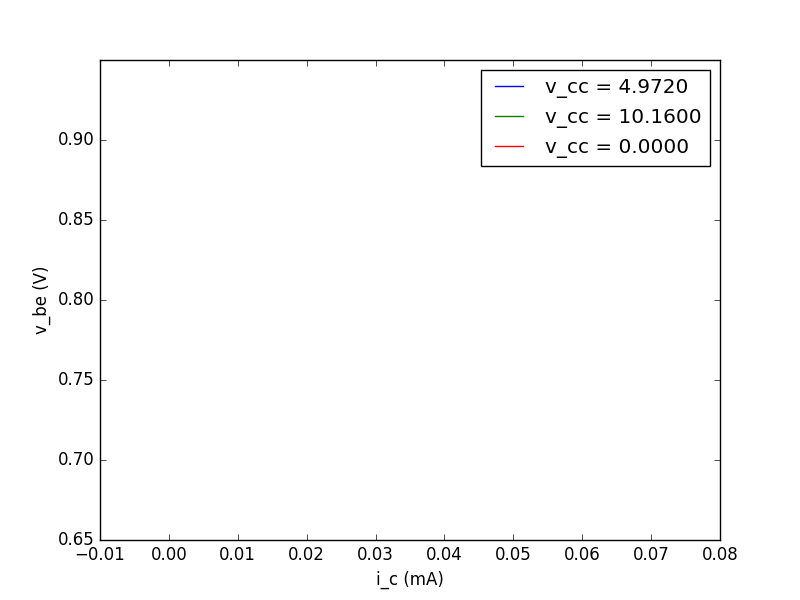
\includegraphics[width=0.6\textwidth]{figs/rel5/v_be.png}
    \caption{Gráfico da corrente $I_C$ em função de $V_{BE}$.}
\end{figure}

\begin{figure}[H]
    \centering
    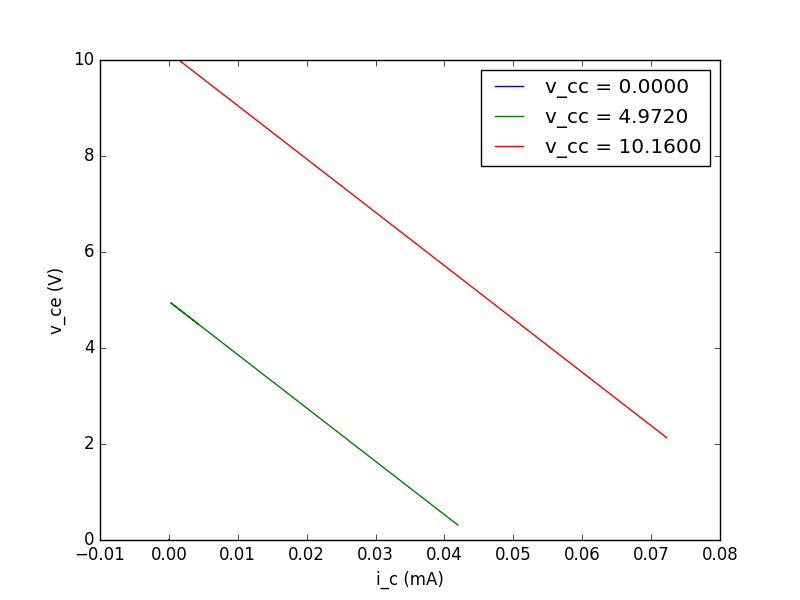
\includegraphics[width=0.6\textwidth]{figs/rel6/v_ce.png}
    \caption{Gráfico da corrente $I_C$ em função de $V_{CE}$.}
\end{figure}

\end{document}
